\documentclass{standalone}
\usepackage{tikz}
\usetikzlibrary{patterns, positioning}


\begin{document}
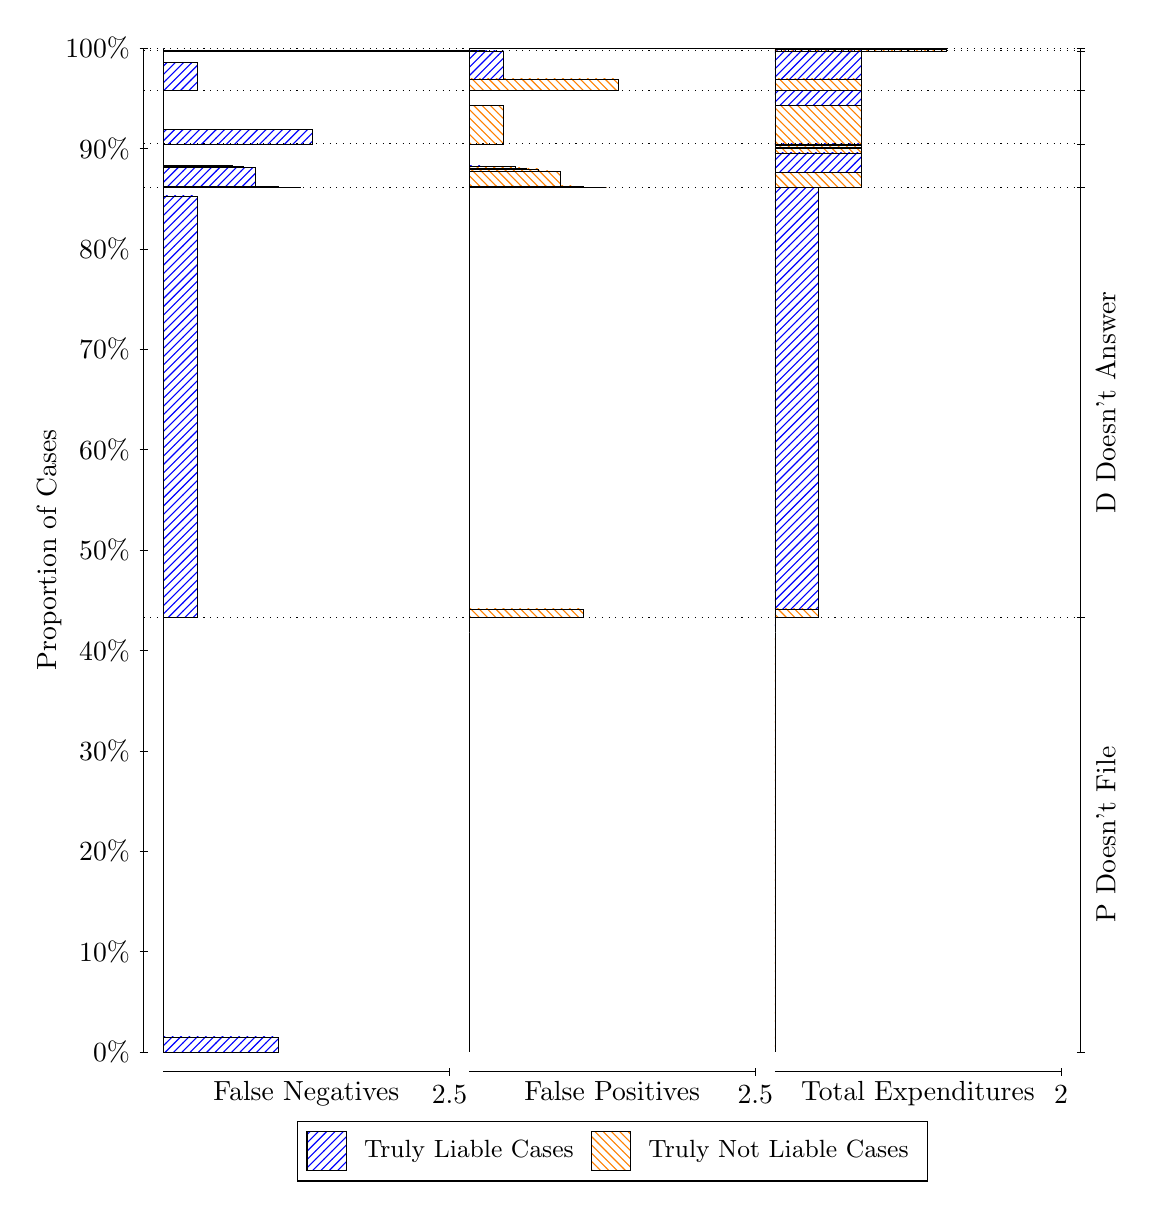
\begin{tikzpicture}
\draw[black, very thin] (1.5,1.75) -- (1.5,14.5);
\node[rotate=90, text=black, anchor=center] at (0.3, 8.125) {Proportion of Cases};
\draw[black, very thin] (1.45,1.75) -- (1.55,1.75);
\node[text=black, anchor=east] at (1.45, 1.75) {0\%};
\draw[black, very thin] (1.45,3.025) -- (1.55,3.025);
\node[text=black, anchor=east] at (1.45, 3.025) {10\%};
\draw[black, very thin] (1.45,4.3) -- (1.55,4.3);
\node[text=black, anchor=east] at (1.45, 4.3) {20\%};
\draw[black, very thin] (1.45,5.575) -- (1.55,5.575);
\node[text=black, anchor=east] at (1.45, 5.575) {30\%};
\draw[black, very thin] (1.45,6.85) -- (1.55,6.85);
\node[text=black, anchor=east] at (1.45, 6.85) {40\%};
\draw[black, very thin] (1.45,8.125) -- (1.55,8.125);
\node[text=black, anchor=east] at (1.45, 8.125) {50\%};
\draw[black, very thin] (1.45,9.4) -- (1.55,9.4);
\node[text=black, anchor=east] at (1.45, 9.4) {60\%};
\draw[black, very thin] (1.45,10.675) -- (1.55,10.675);
\node[text=black, anchor=east] at (1.45, 10.675) {70\%};
\draw[black, very thin] (1.45,11.95) -- (1.55,11.95);
\node[text=black, anchor=east] at (1.45, 11.95) {80\%};
\draw[black, very thin] (1.45,13.225) -- (1.55,13.225);
\node[text=black, anchor=east] at (1.45, 13.225) {90\%};
\draw[black, very thin] (1.45,14.5) -- (1.55,14.5);
\node[text=black, anchor=east] at (1.45, 14.5) {100\%};

\draw[black, very thin] (13.4,1.75) -- (13.4,14.5);
\draw[black, very thin] (13.35,1.75) -- (13.45,1.75);
\node[anchor=west] at (13.35, 1.75) {};
\draw[black, very thin] (13.35,7.2719) -- (13.45,7.2719);
\node[anchor=west] at (13.35, 7.2719) {};
\draw[black, very thin] (13.35,12.728) -- (13.45,12.728);
\node[anchor=west] at (13.35, 12.728) {};
\draw[black, very thin] (13.35,13.282) -- (13.45,13.282);
\node[anchor=west] at (13.35, 13.282) {};
\draw[black, very thin] (13.35,13.963) -- (13.45,13.963);
\node[anchor=west] at (13.35, 13.963) {};
\draw[black, very thin] (13.35,14.465) -- (13.45,14.465);
\node[anchor=west] at (13.35, 14.465) {};
\draw[black, very thin] (13.35,14.491) -- (13.45,14.491);
\node[anchor=west] at (13.35, 14.491) {};
\draw[black, very thin] (13.35,14.5) -- (13.45,14.5);
\node[anchor=west] at (13.35, 14.5) {};

\draw[black, very thin, pattern color=blue, pattern=north east lines] (1.75,1.75) rectangle (3.2033,1.9426);
\draw[black, very thin, pattern color=orange, pattern=north west lines] (1.75,1.9426) rectangle (1.75,7.2719);
\draw[black, very thin, pattern color=blue, pattern=north east lines] (1.75,7.2719) rectangle (2.186,12.621);
\draw[black, very thin, pattern color=orange, pattern=north west lines] (1.75,12.621) rectangle (1.75,12.728);
\draw[black, very thin, pattern color=blue, pattern=north east lines] (1.75,12.728) rectangle (3.494,12.731);
\draw[black, very thin, pattern color=blue, pattern=north east lines] (1.75,12.731) rectangle (3.3487,12.732);
\draw[black, very thin, pattern color=blue, pattern=north east lines] (1.75,12.732) rectangle (3.2033,12.74);
\draw[black, very thin, pattern color=blue, pattern=north east lines] (1.75,12.74) rectangle (3.058,12.741);
\draw[black, very thin, pattern color=blue, pattern=north east lines] (1.75,12.741) rectangle (3.058,12.745);
\draw[black, very thin, pattern color=blue, pattern=north east lines] (1.75,12.745) rectangle (2.9127,12.983);
\draw[black, very thin, pattern color=blue, pattern=north east lines] (1.75,12.983) rectangle (2.7673,12.997);
\draw[black, very thin, pattern color=blue, pattern=north east lines] (1.75,12.997) rectangle (2.622,13.007);
\draw[black, very thin, pattern color=blue, pattern=north east lines] (1.75,13.007) rectangle (2.4767,13.008);
\draw[black, very thin, pattern color=blue, pattern=north east lines] (1.75,13.008) rectangle (2.3313,13.009);
\draw[black, very thin, pattern color=orange, pattern=north west lines] (1.75,13.009) rectangle (1.75,13.282);
\draw[black, very thin, pattern color=blue, pattern=north east lines] (1.75,13.282) rectangle (3.6393,13.471);
\draw[black, very thin, pattern color=orange, pattern=north west lines] (1.75,13.471) rectangle (1.75,13.963);
\draw[black, very thin, pattern color=blue, pattern=north east lines] (1.75,13.963) rectangle (2.186,14.319);
\draw[black, very thin, pattern color=orange, pattern=north west lines] (1.75,14.319) rectangle (1.75,14.465);
\draw[black, very thin, pattern color=blue, pattern=north east lines] (1.75,14.465) rectangle (5.8193,14.466);
\draw[black, very thin, pattern color=orange, pattern=north west lines] (1.75,14.466) rectangle (1.75,14.491);
\draw[black, very thin, pattern color=orange, pattern=north west lines] (1.75,14.491) rectangle (1.75,14.494);
\draw[black, very thin, pattern color=blue, pattern=north east lines] (1.75,14.494) rectangle (1.75,14.5);
\draw[black, very thin, pattern color=orange, pattern=north west lines] (5.6333,1.75) rectangle (5.6333,7.0793);
\draw[black, very thin, pattern color=blue, pattern=north east lines] (5.6333,7.0793) rectangle (5.6333,7.2719);
\draw[black, very thin, pattern color=orange, pattern=north west lines] (5.6333,7.2719) rectangle (7.0867,7.3785);
\draw[black, very thin, pattern color=blue, pattern=north east lines] (5.6333,7.3785) rectangle (5.6333,12.728);
\draw[black, very thin, pattern color=orange, pattern=north west lines] (5.6333,12.728) rectangle (7.3773,12.728);
\draw[black, very thin, pattern color=orange, pattern=north west lines] (5.6333,12.728) rectangle (7.232,12.73);
\draw[black, very thin, pattern color=orange, pattern=north west lines] (5.6333,12.73) rectangle (7.0867,12.74);
\draw[black, very thin, pattern color=orange, pattern=north west lines] (5.6333,12.74) rectangle (6.9413,12.749);
\draw[black, very thin, pattern color=orange, pattern=north west lines] (5.6333,12.749) rectangle (6.796,12.929);
\draw[black, very thin, pattern color=orange, pattern=north west lines] (5.6333,12.929) rectangle (6.6507,12.94);
\draw[black, very thin, pattern color=orange, pattern=north west lines] (5.6333,12.94) rectangle (6.5053,12.964);
\draw[black, very thin, pattern color=orange, pattern=north west lines] (5.6333,12.964) rectangle (6.36,12.977);
\draw[black, very thin, pattern color=orange, pattern=north west lines] (5.6333,12.977) rectangle (6.2147,13);
\draw[black, very thin, pattern color=blue, pattern=north east lines] (5.6333,13) rectangle (5.924,13.001);
\draw[black, very thin, pattern color=blue, pattern=north east lines] (5.6333,13.001) rectangle (5.7787,13.002);
\draw[black, very thin, pattern color=blue, pattern=north east lines] (5.6333,13.002) rectangle (5.6333,13.282);
\draw[black, very thin, pattern color=orange, pattern=north west lines] (5.6333,13.282) rectangle (6.0693,13.774);
\draw[black, very thin, pattern color=blue, pattern=north east lines] (5.6333,13.774) rectangle (5.6333,13.963);
\draw[black, very thin, pattern color=orange, pattern=north west lines] (5.6333,13.963) rectangle (7.5227,14.109);
\draw[black, very thin, pattern color=blue, pattern=north east lines] (5.6333,14.109) rectangle (6.0693,14.465);
\draw[black, very thin, pattern color=orange, pattern=north west lines] (5.6333,14.465) rectangle (5.6333,14.49);
\draw[black, very thin, pattern color=blue, pattern=north east lines] (5.6333,14.49) rectangle (5.6333,14.491);
\draw[black, very thin, pattern color=orange, pattern=north west lines] (5.6333,14.491) rectangle (9.7027,14.494);
\draw[black, very thin, pattern color=blue, pattern=north east lines] (5.6333,14.494) rectangle (8.2493,14.5);
\draw[black, very thin, pattern color=orange, pattern=north west lines] (9.5167,1.75) rectangle (9.5167,7.0793);
\draw[black, very thin, pattern color=blue, pattern=north east lines] (9.5167,7.0793) rectangle (9.5167,7.2719);
\draw[black, very thin, pattern color=orange, pattern=north west lines] (9.5167,7.2719) rectangle (10.062,7.3785);
\draw[black, very thin, pattern color=blue, pattern=north east lines] (9.5167,7.3785) rectangle (10.062,12.728);
\draw[black, very thin, pattern color=orange, pattern=north west lines] (9.5167,12.728) rectangle (10.607,12.92);
\draw[black, very thin, pattern color=blue, pattern=north east lines] (9.5167,12.92) rectangle (10.607,13.169);
\draw[black, very thin, pattern color=orange, pattern=north west lines] (9.5167,13.169) rectangle (10.607,13.23);
\draw[black, very thin, pattern color=blue, pattern=north east lines] (9.5167,13.23) rectangle (10.607,13.243);
\draw[black, very thin, pattern color=orange, pattern=north west lines] (9.5167,13.243) rectangle (10.607,13.263);
\draw[black, very thin, pattern color=blue, pattern=north east lines] (9.5167,13.263) rectangle (10.607,13.282);
\draw[black, very thin, pattern color=orange, pattern=north west lines] (9.5167,13.282) rectangle (10.607,13.774);
\draw[black, very thin, pattern color=blue, pattern=north east lines] (9.5167,13.774) rectangle (10.607,13.963);
\draw[black, very thin, pattern color=orange, pattern=north west lines] (9.5167,13.963) rectangle (10.607,14.109);
\draw[black, very thin, pattern color=blue, pattern=north east lines] (9.5167,14.109) rectangle (10.607,14.465);
\draw[black, very thin, pattern color=orange, pattern=north west lines] (9.5167,14.465) rectangle (11.697,14.49);
\draw[black, very thin, pattern color=blue, pattern=north east lines] (9.5167,14.49) rectangle (11.697,14.491);
\draw[black, very thin, pattern color=orange, pattern=north west lines] (9.5167,14.491) rectangle (11.697,14.494);
\draw[black, very thin, pattern color=blue, pattern=north east lines] (9.5167,14.494) rectangle (11.697,14.5);
\draw[black, dotted] (1.5,7.2719) -- (13.4,7.2719);
\draw[black, dotted] (1.5,12.728) -- (13.4,12.728);
\draw[black, dotted] (1.5,13.282) -- (13.4,13.282);
\draw[black, dotted] (1.5,13.963) -- (13.4,13.963);
\draw[black, dotted] (1.5,14.465) -- (13.4,14.465);
\draw[black, dotted] (1.5,14.491) -- (13.4,14.491);
\draw[black, very thin] (1.75,1.5) -- (5.3833,1.5);
\node[text=black, anchor=north] at (3.5667, 1.5) {False Negatives};
\draw[black, very thin] (5.3833,1.45) -- (5.3833,1.55);
\node[text=black, anchor=north] at (5.3833, 1.45) {2.5};

\draw[black, very thin] (5.6333,1.5) -- (9.2667,1.5);
\node[text=black, anchor=north] at (7.45, 1.5) {False Positives};
\draw[black, very thin] (9.2667,1.45) -- (9.2667,1.55);
\node[text=black, anchor=north] at (9.2667, 1.45) {2.5};

\draw[black, very thin] (9.5167,1.5) -- (13.15,1.5);
\node[text=black, anchor=north] at (11.333, 1.5) {Total Expenditures};
\draw[black, very thin] (13.15,1.45) -- (13.15,1.55);
\node[text=black, anchor=north] at (13.15, 1.45) {2};

\node[text=black, centered, rotate=90] at (13.72, 4.5109) {P Doesn't File};
\node[text=black, centered, rotate=90] at (13.72, 9.9997) {D Doesn't Answer};






\draw (7.449999999999999,1.5) node[draw=none] (baseCoordinate) {};
\begin{scope}[align=center]
        \matrix[scale=0.5, draw=black, below=0.5cm of baseCoordinate, nodes={draw}, column sep=0.1cm]{
            \node[rectangle, draw, minimum width=0.5cm, minimum height=0.5cm, pattern color=blue, pattern=north east lines] {}; &
            \node[draw=none, font=\small, text=black] (B) {Truly Liable Cases}; &
            \node[rectangle, draw, minimum width=0.5cm, minimum height=0.5cm, pattern color=orange, pattern=north west lines] {}; &
            \node[draw=none, font=\small, text=black] (B) {Truly Not Liable Cases}; \\
            };
\end{scope}

\end{tikzpicture}
\end{document}